\section{The trace anomaly at a turning point}\label{rep:trace}

A contracting flat universe turns around only if, at the instant $H=0$, its total energy is non-positive and its trace is sufficiently negative.
We show that the trace anomaly forbids conformal matter alone to meet the second condition when the universe is anisotropic.
At every anisotropic zero of $H$, $\dot H\leq-5S/54$ in any state of a conformal field theory inside the conformal collider bounds, Eq.~\eqref{eq:rA-rate}. %
A turning point therefore needs matter with equation of state $w<1/3$, and a positive potential supplies the missing trace most cheaply.
The chapter derives the curvature invariants of Bianchi~I from scratch (Sec.~\ref{rA:curvature}), completes the square that the anomaly forms at a turning point (Sec.~\ref{rA:square}), proves the obstruction and the rate bound (Sec.~\ref{rA:obstruction}), excludes degenerate crossings (Sec.~\ref{rA:hidentity}) and computes what other matter must supply (Sec.~\ref{rA:supply}).
Only assumption~\ref{assump:A1} and the hypotheses stated with each result are used.

\subsection{Kinematics of a turning point}
\label{rA:kinematics}

Einstein's equations for the homogeneous metric~\eqref{eq:rA-metric}, derived in Sec.~\ref{rA:geometry}, are
\begin{equation}
3\MPbar^2H^2=\rho+\tfrac12\MPbar^2S,\qquad \dot H=-\frac{\rho+\bar p}{2\MPbar^2}-\tfrac12S .
\label{eq:rA-tr-einstein}
\end{equation}
At a turning point $H=0$.
The constraint then fixes the energy density, $\rho=-\tfrac12\MPbar^2S$, and inserting $S=-2\rho/\MPbar^2$ into the second equation gives
\begin{equation}
\dot H\big|_{H=0}=-\frac{\rho+\bar p}{2\MPbar^2}+\frac{\rho}{\MPbar^2}=\frac{\rho-\bar p}{2\MPbar^2}.
\label{eq:rA-hdot-turn}
\end{equation}
A bounce, $\dot H>0$, therefore requires $\bar p<\rho$.
With $T=-\rho+3\bar p$ the inequality $\bar p<\rho$ is equivalent to $T<-\rho+3\rho=2\rho=-\MPbar^2S$, so that~\cite{Solomons:2001ef}
\begin{equation}
\bar p<\rho=-\tfrac12\MPbar^2S\leq0\quad\Longleftrightarrow\quad T<-\MPbar^2S .
\label{eq:rA-trace-criterion}
\end{equation}
The total energy must be non-positive and the trace sufficiently negative.

The first condition has a counterpart in the null geometry of Bianchi~I.
For a null geodesic with frequency $\omega_p$ measured by the comoving observers, the optical tensor of the congruence, the expansion and shear of its transverse cross section, is the projection of $\omega_p\mathsf K$ onto the screen.
At an isotropic turning point the optical tensor of every null congruence therefore vanishes, $B_p=\omega_pH\,\rAone_2=0$.
In the language of Ref.~\cite{Zhou:2026szo}, every null direction is then saturated at that instant, and Lemma~5.1 of that reference states that the total energy at a saturated instant is non-positive.
Equation~\eqref{eq:rA-trace-criterion} adds the trace condition that a dynamical turn needs.
The rest of this chapter asks who can pay for the trace.

\subsection{Curvature invariants of Bianchi~I}
\label{rA:curvature}

The trace of conformal matter depends on the Weyl tensor and the Euler density, so we first compute both for the metric~\eqref{eq:rA-metric} without assuming a diagonal $\mathsf K$ or commuting shear.
Let $K_{ij}=\tfrac12\dot h_{ij}$, $\mathsf K^i{}_j=h^{ik}K_{kj}$ and $\mathcal V=(\det h)^{1/2}$.

\paragraph{Gauss--Codazzi.}
The slices are flat and $K_{ij}$ depends on $t$ only, so the Gauss and Codazzi relations give
\begin{equation}
R_{ijkl}=K_{ik}K_{jl}-K_{il}K_{jk},\qquad R_{0ijk}=0,\qquad R_{0i0j}=-\big(\dot K_{ij}-K_{ik}\mathsf K^k{}_j\big).
\label{eq:rA-gauss}
\end{equation}
The last relation follows from the geodesic deviation of the comoving observers: the separation vector $\xi$ obeys $\nabla_u\xi=\mathsf K\xi$, and the second derivative gives the tidal matrix $R^i{}_{0j0}=-(\dot{\mathsf K}+\mathsf K^2)^i{}_j$.
Lowering the index with $h_{ij}$ and using $h_{ik}\dot{\mathsf K}^k{}_j=\dot K_{ij}-2K_{ik}\mathsf K^k{}_j$ gives the form quoted.

\paragraph{Frame components.}
We now use an orthonormal frame transported along the comoving geodesics.
Because $\Gamma^i_{tk}=\mathsf K^i{}_k$, the covariant time derivative of the mixed tensor $\mathsf K$ equals its ordinary derivative, $(\nabla_t\mathsf K)^i{}_j=\dot{\mathsf K}^i{}_j$, so the frame components of $\mathsf K$ obey the same equations as the mixed components.
We write
\begin{equation}
\mathsf K=H\rAone+\sigma,\qquad u\equiv\dot\sigma,\qquad P\equiv\sigma^2-\tfrac13S\,\rAone ,
\label{eq:rA-uP}
\end{equation}
where $\sigma$ and $u$ are symmetric and trace free but need not commute.
The characteristic polynomial of a trace-free $3\times3$ matrix gives $\sigma^3=\tfrac12S\,\sigma+(\det\sigma)\rAone$, hence $\Tr\sigma^3=3\det\sigma$ and
\begin{equation}
\Tr\sigma^4=\tfrac12S^2,\qquad \Tr P^2=\Tr\sigma^4-\tfrac23S^2+\tfrac13S^2=\tfrac16S^2,\qquad \Tr(\sigma P)=\Tr\sigma^3 .
\label{eq:rA-cayley}
\end{equation}

\paragraph{Ricci tensor.}
In the frame, Eq.~\eqref{eq:rA-gauss} gives $R_{0i0j}=-(\dot{\mathsf K}+\mathsf K^2)_{ij}$ and $R^k{}_{ikj}=(\Tr\mathsf K)\,\mathsf K_{ij}-(\mathsf K^2)_{ij}$.
Hence
\begin{equation}
\begin{aligned}
R_{00}&=-\Tr\big(\dot{\mathsf K}+\mathsf K^2\big)=-\big(3\dot H+3H^2+S\big),\\
R_{ij}&=\big(\dot{\mathsf K}+(\Tr\mathsf K)\mathsf K\big)_{ij}=\big(\dot H+3H^2\big)\delta_{ij}+u_{ij}+3H\sigma_{ij},\\
R&=-R_{00}+\Tr R_{ij}=6\dot H+12H^2+S .
\end{aligned}
\label{eq:rA-ricci}
\end{equation}
With $R_{00}=(\rho+3\bar p)/2\MPbar^2$ the first line is Raychaudhuri's equation used in Eq.~\eqref{eq:rA-einstein}.

\paragraph{Weyl tensor.}
The electric part of the Weyl tensor follows from $C_{0i0j}=R_{0i0j}+\tfrac12R_{ij}-\tfrac12\delta_{ij}R_{00}-\tfrac16R\,\delta_{ij}$, which is the decomposition of the Riemann tensor in four dimensions evaluated in the frame.
Inserting Eq.~\eqref{eq:rA-ricci}, the terms in $\dot H$ and $H^2$ cancel, and
\begin{equation}
E_{ij}\equiv C_{0i0j}=-\tfrac12u-\tfrac12H\sigma-\sigma^2+\tfrac13S\rAone=-\tfrac12\big(u+H\sigma+2P\big)_{ij}.
\label{eq:rA-electric}
\end{equation}
The magnetic part $B_{ij}=\tfrac12\epsilon_{ikl}C^{kl}{}_{0j}$ is built from $R_{0ijk}$ and from spatial gradients of $\mathsf K$, and vanishes for a homogeneous flat slicing.
Since $C_{abcd}C^{abcd}=8(E_{ij}E^{ij}-B_{ij}B^{ij})$,
\begin{equation}
W^2=2\Tr\big(u+H\sigma+2P\big)^2 .
\label{eq:rA-W2}
\end{equation}

\paragraph{Euler density.}
For Bianchi~I the Euler density is a total derivative,
\begin{equation}
E_4=R_{abcd}R^{abcd}-4R_{ab}R^{ab}+R^2=\frac{8}{\mathcal V}\,\frac{d}{dt}\big(\mathcal V\det\mathsf K\big).
\label{eq:rA-E4total}
\end{equation}
With $\det\mathsf K=H^3-\tfrac12HS+\tfrac13\Tr\sigma^3$, $\dot{\mathcal V}=3H\mathcal V$, $\dot S=2\Tr(u\sigma)$ and $\tfrac{d}{dt}\tfrac13\Tr\sigma^3=\Tr(\sigma^2u)=\Tr(uP)$, Eq.~\eqref{eq:rA-E4total} becomes
\begin{equation}
E_4=24H^4+24H^2\dot H-\big(12H^2+4\dot H\big)S-8H\Tr(u\sigma)+8\Tr(uP)+8H\Tr\sigma^3 .
\label{eq:rA-E4}
\end{equation}
For flat Friedmann--Robertson--Walker cosmologies, $\sigma=u=0$, this reduces to $E_4=24H^2(\dot H+H^2)$.
An independent route is $E_4=W^2-2R_{ab}R^{ab}+\tfrac23R^2$ with Eqs.~\eqref{eq:rA-ricci} and~\eqref{eq:rA-W2}; the two expressions agree identically.
We checked these identities symbolically for unrestricted trace-free symmetric matrices, and numerically from the coordinate Riemann tensor of 500 random metric jets with noncommuting shear; the largest scaled error is $4.9\times10^{-14}$. %

At a turning point, $H=0$, the invariants reduce to
\begin{equation}
W^2=2\Tr(u+2P)^2,\qquad E_4=-4\dot HS+8\Tr(uP),\qquad \Tr P^2=\tfrac16S^2 .
\label{eq:rA-invH0}
\end{equation}

\subsection{The anomaly completes a square}
\label{rA:square}

In this chapter the light fields form a conformal field theory (CFT) with anomaly coefficients $a,c>0$.
Its trace is fixed by the curvature in every state~\cite{Duff:1993wm},
\begin{equation}
\langle T^\mu{}_\mu\rangle=\frac{cW^2-aE_4}{16\pi^2}+b\,\Box R ,
\label{eq:rA-anomaly}
\end{equation}
where $W^2$ is the square of the Weyl tensor and $E_4$ the Euler density.
In this normalization a real scalar has $(c,a)=(\tfrac1{120},\tfrac1{360})$, a Weyl fermion $(\tfrac1{40},\tfrac{11}{720})$ and a Maxwell field $(\tfrac1{10},\tfrac{31}{180})$.

At $H=0$, Eq.~\eqref{eq:rA-invH0} gives
\begin{equation}
cW^2-aE_4=2c\Tr u^2+8(c-a)\Tr(uP)+8c\Tr P^2+4a\dot HS .
\label{eq:rA-cWaE}
\end{equation}
The Euler density contributes the indefinite cross term $-8a\Tr(uP)$, which a positive Weyl square must absorb.
With $\varrho\equiv a/c$, the square
\begin{equation}
2c\Tr\big[u-2(\varrho-1)P\big]^2=2c\Tr u^2-8(a-c)\Tr(uP)+8c(\varrho-1)^2\Tr P^2
\end{equation}
reproduces the first two terms of Eq.~\eqref{eq:rA-cWaE}, and the remainder is $8c[1-(\varrho-1)^2]\Tr P^2=\tfrac43c\,\varrho(2-\varrho)S^2$.
Hence
\begin{equation}
\begin{aligned}
cW^2-aE_4&=Q_0+4a\dot HS,\\
Q_0&=2c\Tr[u-2(\varrho-1)P]^2+\tfrac{4a}{3}(2-\varrho)S^2 .
\end{aligned}
\label{eq:rA-square}
\end{equation}
The matrix $u-2(\varrho-1)P$ is real and symmetric, so its square has a non-negative trace.
For $\varrho\leq2$ the Weyl square therefore absorbs the indefinite Euler term, and $Q_0\geq0$.
The anomaly enters the dynamics of $\dot H$ only through the explicit term $4a\dot HS$; everything else is the non-negative $Q_0$.

\subsection{Obstruction and rate bound}
\label{rA:obstruction}

\paragraph{The $\Box R$ term.}
A finite local counterterm $\alpha R^2$ in the gravitational action contributes $\propto\alpha\,\Box R$ to the trace, so the coefficient $b$ is shifted by a choice of renormalization scheme.
We take the net $b$ to vanish; a healthy $R^2$ term with $b\neq0$ is discussed at the end of the chapter.

\paragraph{Traced Einstein equation.}
The trace of $\MPbar^2G_{\mu\nu}=\langle T_{\mu\nu}\rangle$ is $-\MPbar^2R=\langle T^\mu{}_\mu\rangle$.
Let $T_{\rm extra}$ be the trace of all matter other than the CFT.
At $H=0$, $R=6\dot H+S$ by Eq.~\eqref{eq:rA-ricci}, and with Eq.~\eqref{eq:rA-square}
\begin{equation}
-\MPbar^2\big(6\dot H+S\big)=\frac{Q_0+4a\dot HS}{16\pi^2}+T_{\rm extra}.
\end{equation}
The equation is algebraic in $\dot H$:
\begin{equation}
\dot H=-\frac{\MPbar^2S+Q_0/16\pi^2+T_{\rm extra}}{6\MPbar^2+aS/4\pi^2}.
\label{eq:rA-hdot}
\end{equation}
Only the state-independent trace enters; the CFT energy density and anisotropic stress drop out of Eq.~\eqref{eq:rA-hdot}, although they enter the constraint and the evolution of $\sigma$.

\begin{rAtheorem}[Obstruction]\label{thm:rA-obstruction}
Let the light fields form a CFT with $0<a\leq2c$, let all other matter have non-negative trace, $T_{\rm extra}\geq0$, and let $b=0$.
Then a contracting universe with metric~\eqref{eq:rA-metric} cannot turn around: at every zero of $H$ with $S>0$, $\dot H<0$, and no regular solution passes from $H<0$ to $H>0$.
\end{rAtheorem}

\begin{rAproof}
At a zero of $H$ the numerator of Eq.~\eqref{eq:rA-hdot} is at least $\MPbar^2S$, because $Q_0\geq0$ for $\varrho\leq2$ and $T_{\rm extra}\geq0$, and the denominator is positive.
Hence $\dot H\leq-\MPbar^2S/(6\MPbar^2+aS/4\pi^2)<0$ when $S>0$.
At an isotropic zero, $S=0$, the same equation gives only $\dot H\leq0$, and the possibility of a degenerate crossing is excluded by Lemma~\ref{lem:rA-crossing} below, which uses the identity for general $H$.
\end{rAproof}

Neither negative CFT energy nor a large anisotropic CFT stress helps, because neither enters Eq.~\eqref{eq:rA-hdot}.
The hypothesis $a\leq2c$ holds for every unitary, parity-preserving CFT: positivity of the energy flux measured in collider-type experiments, the conformal collider bounds, restricts such theories to $\tfrac13\leq a/c\leq\tfrac{31}{18}$~\cite{Hofman:2008ar,Hofman:2016awc}.
The free fields saturate or lie inside the bounds: $\varrho=\tfrac13$ for a conformal scalar, $\tfrac{11}{18}$ for a Dirac fermion and $\tfrac{31}{18}$ for a Maxwell field.
For the Standard Model at the turn, four real scalars, 45 Weyl fermions and twelve vectors,
\begin{equation}
c=\frac{4+135+144}{120}=\frac{283}{120},\qquad a=\frac{4+247.5+744}{360}=\frac{995.5}{360},\qquad \frac ac=1.17,
\label{eq:rA-SMac}
\end{equation}
inside the collider bound $31/18$. %

\paragraph{Rate bound.}
The obstruction becomes quantitative when we minimize $Q_0$ over the free data $u$.
The minimum, $u=2(\varrho-1)P$, gives $Q_0\geq\tfrac43a(2-\varrho)S^2$.
With the anomaly strength
\begin{equation}
y\equiv\frac{aS}{24\pi^2\MPbar^2},
\end{equation}
the denominator of Eq.~\eqref{eq:rA-hdot} is $6\MPbar^2(1+y)$ and the minimal $Q_0/16\pi^2$ is $2(2-\varrho)y\,\MPbar^2S$, so that for $T_{\rm extra}\geq0$
\begin{equation}
\frac{\dot H}{S}\leq-\frac{1+2(2-\varrho)y}{6(1+y)} .
\end{equation}
At the upper collider bound, $\varrho=\tfrac{31}{18}$, $2(2-\varrho)=\tfrac59$, and writing $1+\tfrac59y=\tfrac59(1+y)+\tfrac49$ gives
\begin{equation}
\frac{\dot H}{S}\leq-\frac{1+2(2-\varrho)y}{6(1+y)}\leq-\frac5{54}-\frac{2}{27(1+y)},
\label{eq:rA-rate}
\end{equation}
so that $\dot H\leq-5S/54$ at every anisotropic zero of $H$, in any state and at any coupling [Fig.~\ref{fig:rA-trace}(a)]. %

\paragraph{Rotating shear axes.}
If the principal axes of the shear rotate, they only strengthen the bound.
Write $\sigma=O\,{\rm diag}(s_1,s_2,s_3)\,O^{\mathsf T}$ with principal shears $s_i$ and a rotation $O(t)$, and let $\Xi=O^{\mathsf T}\dot O$, an antisymmetric matrix, be the rotation rate of the principal frame.
Then $u=O\big[{\rm diag}(\dot s_i)+[\Xi,{\rm diag}(s_i)]\big]O^{\mathsf T}$, and the commutator has the off-diagonal entries $\Xi_{ij}(s_j-s_i)$, while $P$ is diagonal in the principal frame.
The trace of the square splits into a diagonal and an off-diagonal part, and the latter adds
\begin{equation}
\Delta Q_0=4c\sum_{i<j}(s_i-s_j)^2\,\Xi_{ij}^2\geq0
\end{equation}
to $Q_0$; a numerical check of the split agrees to $2\times10^{-15}$. %

\paragraph{Isotropic turning points.}
At an isotropic turning point of an isotropic history, where also $u=0$, the anomaly terms of Eq.~\eqref{eq:rA-hdot} vanish, as they do at the turning points of the anomaly-corrected Friedmann equation of an isotropic Casimir torus~\cite{Mithani:2014toa}.
The strict rate bound~\eqref{eq:rA-rate} is a property of anisotropic turning points.

\begin{figure}[tbp]
\centering
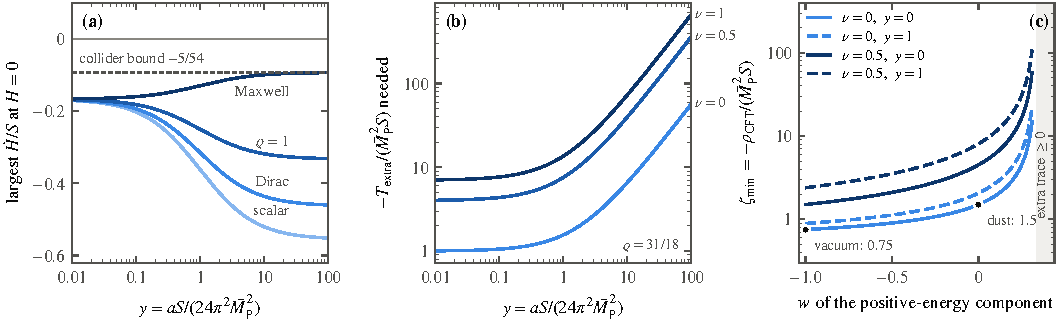
\includegraphics[width=\textwidth]{prd_trace}
\caption{Trace requirements at an anisotropic turning point.
(a)~Largest $\dot H/S$ at a zero of $H$ when all other matter has non-negative trace, Eq.~\eqref{eq:rA-rate}, versus the anomaly strength $y$, for $\varrho=a/c$ of a conformal scalar ($\tfrac13$), a Dirac fermion ($\tfrac{11}{18}$), a Maxwell field ($\tfrac{31}{18}$), and $\varrho=1$; every curve stays below $-5/54$. %
(b)~Least negative extra trace needed for a turning rate $\nu=\dot H/S$ at $\varrho=\tfrac{31}{18}$, Eq.~\eqref{eq:rA-budget}.
(c)~Least negative CFT energy $\zeta_{\min}$, Eq.~\eqref{eq:rA-joint}, when a positive-energy component with equation of state $w$ supplies the trace; for $w\geq1/3$ (shaded) the obstruction applies.}
\label{fig:rA-trace}
\end{figure}

\subsection{The zero-expansion boundary}
\label{rA:hidentity}

The obstruction at $S>0$ is strict, but an isotropic zero of $H$ with $\dot H=0$ is degenerate, and we must exclude a crossing through it.
For this we need the anomaly at general $H$.
Inserting Eqs.~\eqref{eq:rA-W2} and~\eqref{eq:rA-E4} without setting $H=0$, and collecting the terms that do not vanish at $H=0$ into $Q_0+4a\dot HS$, gives
\begin{equation}
\begin{aligned}
cW^2-aE_4&=Q_0+4a\dot H\big(S-6H^2\big)+H\mathcal P,\\
\mathcal P&=4(c+2a)\Tr(u\sigma)+8(c-a)\Tr\sigma^3+(2c+12a)HS-24aH^3 .
\end{aligned}
\label{eq:rA-genH}
\end{equation}
The four terms of $\mathcal P$ come from $4cH\Tr(u\sigma)+8aH\Tr(u\sigma)$, from $8cH\Tr\sigma^3-8aH\Tr\sigma^3$, from $2cH^2S+12aH^2S$ and from $-24aH^4$; the term $-24aH^2\dot H$ joins $4a\dot HS$.
With $R=6\dot H+12H^2+S$ and $b=0$ the traced Einstein equation reads
\begin{equation}
\Big[6\MPbar^2+\frac{a(S-6H^2)}{4\pi^2}\Big]\dot H=-\MPbar^2\big(12H^2+S\big)-\frac{Q_0+H\mathcal P}{16\pi^2}-T_{\rm extra}.
\label{eq:rA-genH-trace}
\end{equation}

\begin{rAlemma}[No degenerate crossing]\label{lem:rA-crossing}
Under the hypotheses of Theorem~\ref{thm:rA-obstruction}, a regular contracting solution cannot cross $H=0$, even at a degenerate zero with $\dot H(t_*)=0$.
\end{rAlemma}

\begin{rAproof}
Near a regular zero of $H$ the bracket on the left of Eq.~\eqref{eq:rA-genH-trace} exceeds $3\MPbar^2$, since it equals $6\MPbar^2+aS/4\pi^2$ at $H=0$ and is continuous.
With $\varrho\leq2$ and $T_{\rm extra}\geq0$ every term on the right except $-H\mathcal P/16\pi^2$ is non-positive, and $\mathcal P$ is bounded on a compact neighborhood of $t_*$.
Hence $\dot H\leq k|H|$ there, for a constant $k$.
If $H$ became positive after a zero at $t_*$, then $d(e^{-kt}H)/dt=e^{-kt}(\dot H-kH)\leq0$ wherever $H>0$, so $e^{-kt}H(t)\leq e^{-kt_*}H(t_*)=0$ on the first interval of positivity, a contradiction.
\end{rAproof}

The lemma completes the proof of Theorem~\ref{thm:rA-obstruction}.
Numerically, Eq.~\eqref{eq:rA-genH} holds to $10^{-12}$ in relative terms for random noncommuting $\sigma$ and $u$ and random $H$, $\dot H$, $a$ and $c$. %

\subsection{What a turning point must supply}
\label{rA:supply}

Allowing any $T_{\rm extra}$, we now ask how negative it must be.
Setting $\dot H=\nu S$ with a turning rate $\nu>0$ in Eq.~\eqref{eq:rA-hdot} and solving for $T_{\rm extra}$ gives $-T_{\rm extra}=\MPbar^2S+Q_0/16\pi^2+6\nu\MPbar^2S(1+y)$.
With the minimal $Q_0$ and the collider bound,
\begin{equation}
-\frac{T_{\rm extra}}{\MPbar^2S}\geq1+6\nu(1+y)+2(2-\varrho)y\geq1+6\nu(1+y)+\frac59y .
\label{eq:rA-budget}
\end{equation}

\paragraph{Who pays.}
Suppose that a positive-energy component with $\bar p=w\rho_w$ supplies the trace, $T_{\rm extra}=-(1-3w)\rho_w$, and the CFT supplies the energy $\rho_{\rm CFT}=-\zeta\MPbar^2S$.
The constraint at the turn, $\rho_w+\rho_{\rm CFT}=-\tfrac12\MPbar^2S$, fixes $\rho_w=(\zeta-\tfrac12)\MPbar^2S$, and Eq.~\eqref{eq:rA-budget} becomes $(\zeta-\tfrac12)(1-3w)\geq1+6\nu(1+y)+5y/9$.
For $w<1/3$ this gives
\begin{equation}
\zeta\geq\frac12+\frac{1+6\nu(1+y)+5y/9}{1-3w}.
\label{eq:rA-joint}
\end{equation}
For $w\geq1/3$ no positive $\rho_w$ satisfies the inequality, and the obstruction applies.
At marginal turning, $\nu\to0$, the least negative CFT energy is $\zeta=\tfrac34+\tfrac{5}{36}y$ for vacuum energy, $w=-1$, and $\tfrac32+\tfrac59y$ for dust, $w=0$ [Fig.~\ref{fig:rA-trace}(c)]. %
Any positive-energy matter with $w<1/3$ can pay for the trace.
Vacuum energy does it most cheaply, while saturating the null energy condition, so the most economical turning point combines a positive potential with a separate source of negative energy.

\paragraph{An exact criterion.}
With $T_{\rm extra}=-4\rho_\Lambda$ and $\rho_\Lambda=3\MPbar^2h^2$, the numerator of Eq.~\eqref{eq:rA-hdot} is $\MPbar^2S+Q_0/16\pi^2-12\MPbar^2h^2$, and Eq.~\eqref{eq:rA-hdot} becomes an exact criterion for every state of the conformal sector:
\begin{equation}
\dot H>0\quad\Longleftrightarrow\quad S_b<12h^2-\frac{Q_0}{16\pi^2\MPbar^2},
\label{eq:rA-exact-criterion}
\end{equation}
where $S_b$ is the shear at the turn.
For a rolling inflaton, $\rho_\phi=K_\phi+V$ and $\bar p_\phi=K_\phi-V$ with $K_\phi=\tfrac12\dot\phi^2$, so $-T_{\rm extra}=4V-2K_\phi$, and the kinetic energy of the inflaton counts against the turn.
For the Casimir turning point of Sec.~\ref{rep:turning} the shear and $Q_0$ vanish at the turn of the isotropic background, and Eq.~\eqref{eq:rA-exact-criterion} holds with a margin $12h^2$; anomalous corrections to it are of relative order $\epsilon^2$, with $\epsilon\simeq3\times10^{-5}$ the small parameter of Sec.~\ref{rep:turning}. %

\paragraph{Beyond the conformal hypothesis.}
Running couplings, masses or minimally coupled scalars break the conformal hypothesis~\cite{CesareSilva:2024nym,CesareSilva:2026zne}, and a healthy $R^2$ term shifts $b$ and requires negative matter energy~\cite{Anderson:1983nq,DeFelice:2010aj}.
The rest of this report takes the most economical route: a positive potential (assumption~\ref{assump:A3}) and the negative Casimir energy of the Standard Model, computed in the next chapter.
